%\linenumbers*
\chapter{FURTHER STUDY ON TEMPORAL INTENSITY VARIATION}
\label{chap:bp2bpvariationchapter}
%need better title. more specific rather than further study

\section{Aim}
\label{sec:Aim}
This experiment is to investigate impacts of \emph{temporal intensity
variations} on runoff and soil loss generations using WEPP and EUROSEM.

The questions I would like to address here are:
\begin{enumerate}
  \item Why do we need rainfall data with higher temporal resolution for erosion
modelling?
  \item Then, how high is high enough resolution for erosion modelling?
% \item What are \% changes from the constant (baseline) rainfall?
\end{enumerate}

\section{Method}
\label{sec:Method}

\begin{table}[htbp]
  \figureversion{tabular}
  \centering
  \small
  \caption{Two examples of rainstorms}
  \label{tab:TwoExamplesofRainstorm}
    \begin{tabular}{ccc}
    \toprule
     Time (min) & Storm A & Storm B \\
    \midrule
%    0 &  &  \\
    1 & 3 & 1 \\
    2 & 4 & 3 \\
    3 & 8 & 2 \\
    4 & 15 & 4 \\
    5 & 6 & 6 \\
    6 & 8 & 3 \\
    7 & 5 & 3 \\
    8 & 3 & 7 \\
    9 &  & 4 \\
    10&  & 5 \\
    11&  & 3 \\
    12&  & 5 \\
    13&  & 2 \\
    14&  & 3 \\
    15&  & 1 \\
    \bottomrule
    \end{tabular}
\end{table}

\begin{figure}[htbp]
  \centering
    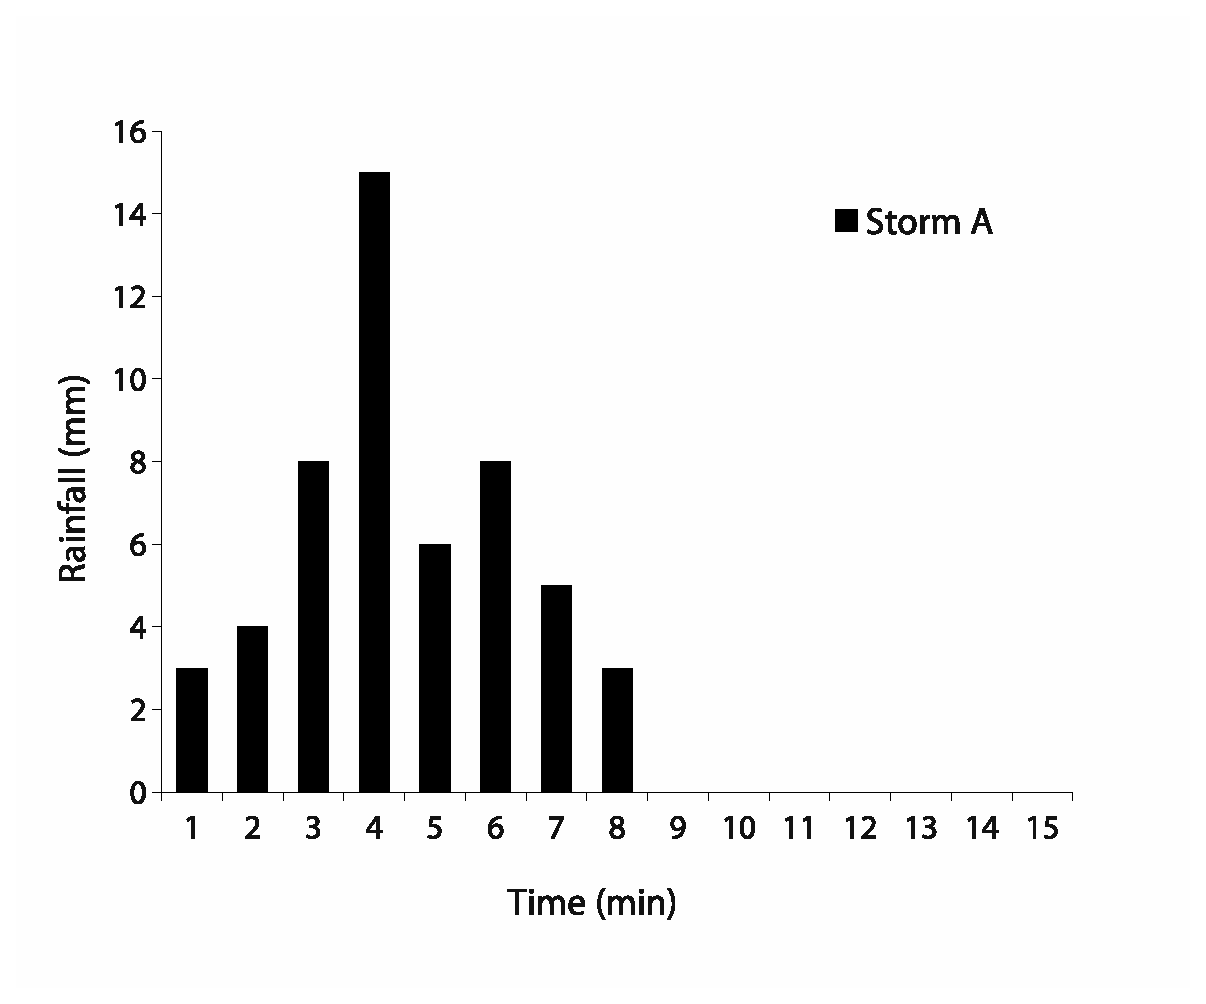
\includegraphics[width=0.49\textwidth]{./img/example_storm_a}
    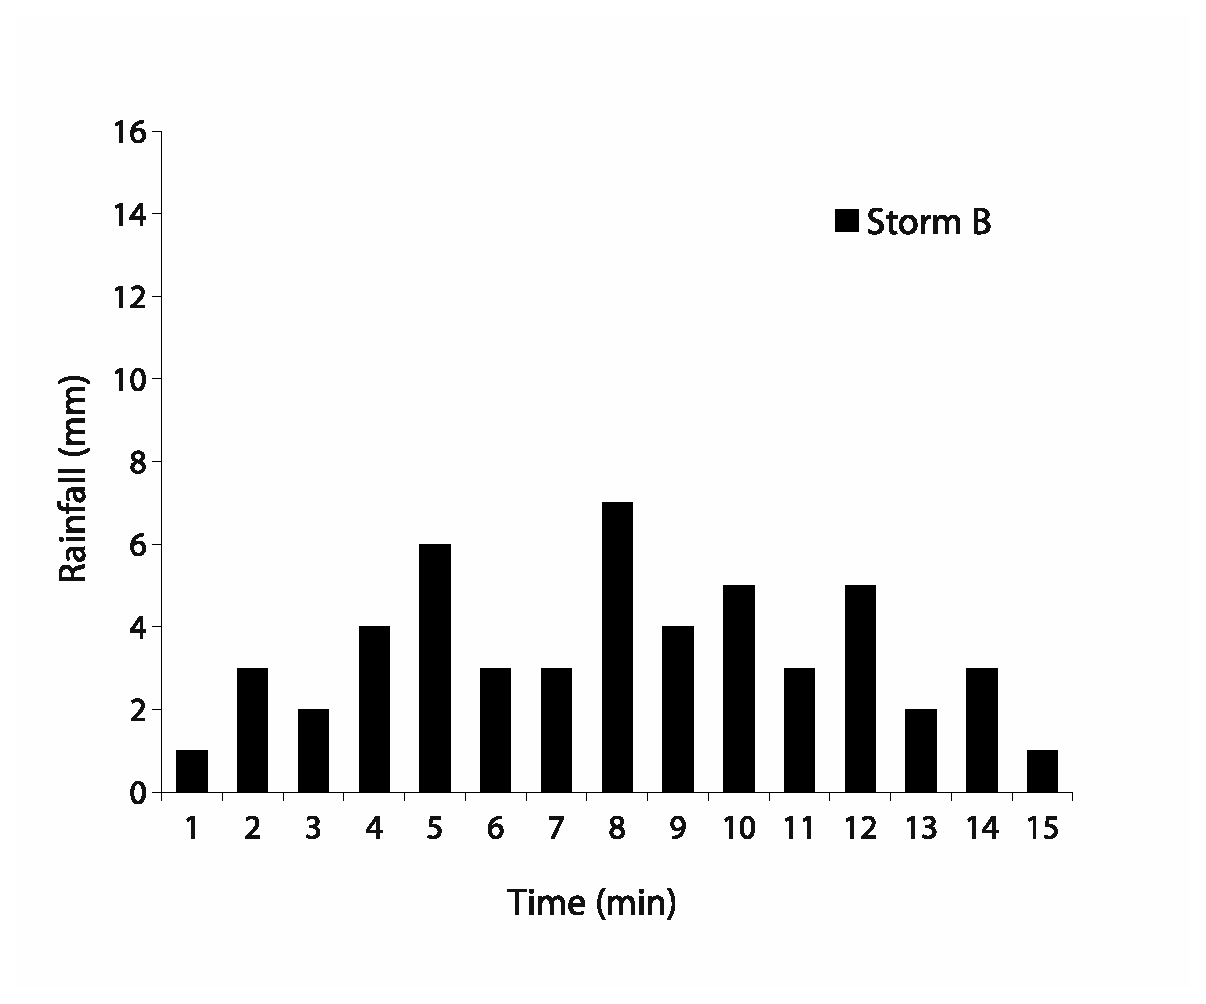
\includegraphics[width=0.49\textwidth]{./img/example_storm_b}
  \caption{Two examples of rainstorms}
  \label{fig:TwoExamplesofRainstorm}
\end{figure}

\begin{itemize}
  \item Take BP data of both rain storms (July + October) -- only October storm
for the moment.
  \item Starting from 15-min (since 1- and 5-min are not possible for WEPP and
EUROSEM because of too many breakpoints) to 60-min. (i.e. 15-, 30-, 60-min data)
  \item Original data may have high temporal variability between breakpoint to
breakpoint.
    \begin{itemize}
      \item Let's assume that we only can record rainfall data with a single
fixed temporal resolution, say 15-min to start with.
      \item When intensity changes rapidly, temporal variability of the
intensity between BP to BP is high, so that higher temporal resolution
\emph{may} be required.
      \item On the other hand, when intensity changes slowly, temporal
variability of the intensity between BP to BP will be low. Therefore, higher
temporal resolution \emph{may not} be required.
    \end{itemize}
  \item Sort data to ``ascending'' (Sorted-ascending) and ``descending''
(Sorted-descending) order to reduce the temporal variability. This means the
sorted data will not have any no-rain phases within the storm duration. Thus,
no-rain phase in the original rainfall data may also need to be removed to
minimize possible effects from the no-rain phases (Original Rainfall (no-gaps)).
  \item Total rainfall amounts are the same for all the modified data (133.8 mm)
  \item Are the duration also the same? -- no, they are different.
    \begin{itemize}
      \item They are different because all the no-rain periods have been
removed.
      \item Thus, re-sorted data have shorter storm duration compared to
original.
      \item 1215, 1230 and 1260 min for 15-min, 30-min and 60-min original data
      \item 930, 1020 and 1080 min for 15-min, 30-min and 60-min sorted and
original-without-gaps data
    \end{itemize}
\end{itemize}

\section{Result}
\label{sec:SimulationResult}

\begin{enumerate}
  \item When rainfall data is re-sorted, some of the storm character is modified
(shape of the storm and duration). Also, number of breakpoint may need to be
recalculated (not done as it may not be important for this stage -- pilot test
was done, and for the WEPP simulation, it makes a difference because of how WEPP
deals with breakpoint. It re-calculates time of breakpoints!)
    \begin{itemize}
      \item Original data vs. Sorted data (unchanged breakpoints)
      \item Sorted data (unchanged breakpoints) vs. Sorted data (redefined
breakpoints) -- see the comments above.
      \item Original data vs. Sorted data (redefined breakpoints) -- not done,
far from the pilot test.
      \item Thus, resulting runoff and soil loss estimations may differ when BP
was redefined.
      \item For the moment, I only looked at 1? %or may be 3??
    \end{itemize}
  \item October storm
    \begin{itemize}
      \item Original data
        \begin{itemize}
          \item Amount: 133.8 mm
          \item Duration: 1209 min (for 15-min data)
        \end{itemize}
      \item Modified data (ascending, descending and original-without-gaps)
        \begin{itemize}
          \item Amount: 133.8 mm
          \item Duration: 942 min (for 15-min data)
        \end{itemize}
    \end{itemize}
\end{enumerate}

\subsection{WEPP simulation}
\label{sec:WEPPSimulation}

\begin{sidewaystable}[htbp]
  \centering
  \small
  \caption{WEPP simulations with October rainfall data}
  \label{tab:WEPPSimulationsWithOctoberRainfallData}
    \begin{tabular}{llllllllllllll}
\toprule
\multicolumn{3}{c}{WEPP with October Storm} & D & E & F & G & H & I & J & K & L
& MEAN & \% $\Delta$ from original \\
\midrule
15-min & runoff & original & 63.9 & 63.6 & 71.1 & 81.8 & 86.4 & 86.4 & 86.4 &
71.7 & 71.7 & 75.9 &  \\
 & (mm) & original-nogap &  64.8 &  64.4 &  72.3 &  80.8 &  85.0 &  85.0 &  85.0
& 72.7 &  72.7 &  75.9 & \\
 &  & sorted-ascending & 77.2 & 76.9 & 80.6 & 86.1 & 88.6 & 88.6 & 88.6 & 80.8 &
80.8 & 83.1 & 9.5 \\
 &  & sorted-descending & 73.7 &  73.4 &  76.5 &  81.8 &  84.4 &  84.4 &  84.4 &
76.7 &  76.7 &  79.1 &  4.2 \\
 & soil loss & original & 37.7 & 36.8 & 95.3 & 145.2 & 175.3 & 167.6 & 148.2 &
86.8 & 77.5 & 107.8 &  \\
 & (t/ha) & original-nogap &  46.8 &  49.2 &  105.9 & 152.5 & 180.6 & 171.5 &
151.7 & 94.2 &  85.4 &  115.3 & \\
 &  & sorted-ascending & 60.0 & 62.1 & 121.9 & 164.8 & 190.4 & 181.4 & 161.0 &
108.1 & 96.1 & 127.3 & 18.1 \\
 &  & sorted-descending & 50.5 &  52.2 &  109.9 & 155.7 & 181.9 & 173.1 & 153.8
& 101.8 & 90.8 &  118.8 & 10.2 \\
\midrule
30-min & runoff & original & 68.5 & 67.9 & 72.7 & 77.5 & 79.8 & 79.8 & 79.8 &
72.8 & 72.8 & 74.6 &  \\
 & (mm) & original-nogap &  67.5 &  67.2 &  74.8 &  80.9 &  83.1 &  83.1 &  83.1
& 75.2 &  75.2 &  76.7 & \\
 &  & sorted-ascending & 78.0 & 77.7 & 80.1 & 82.3 & 83.5 & 83.5 & 83.5 & 80.2 &
80.2 & 81.0 & 8.6 \\
 &  & sorted-descending & 74.1 &  73.8 &  76.2 &  77.9 &  79.1 &  79.1 &  79.1 &
76.3 &  76.3 &  76.9 &  3.0\\
 & soil loss & original & 45.0 & 43.8 & 101.4 & 141.1 & 165.3 & 154.5 & 141.0 &
92.7 & 83.9 & 107.6 &  \\
 & (t/ha) & original-nogap &  25.2 &  24.6 &  85.9 &  129.3 & 155.1 & 149.1 &
132.5 & 73.8 &  61.4 &  93.0 & \\
 &  & sorted-ascending & 57.0 & 58.5 & 117.1 & 154.7 & 177.3 & 169.4 & 150.6 &
105.8 & 94.9 & 120.6 & 12.1 \\
 &  & sorted-descending & 43.7 &  43.9 &  102.7 & 138.9 & 160.8 & 153.2 & 134.9
& 91.5 &  80.9 &  105.6 &  $-$1.9\\
\midrule
60-min & runoff & original & 69.9 & 69.4 & 74.2 & 76.6 & 77.3 & 77.3 & 77.3 &
74.3 & 74.3 & 74.5 &  \\
 & (mm) & original-nogap &  69.9 &  69.4 &  74.2 &  76.6 &  77.3 &  77.3 &  77.3
& 74.3 &  74.3 &  74.5 & \\
 &  & sorted-ascending & 75.0 & 74.8 & 77.2 & 78.4 & 78.8 & 78.8 & 78.8 & 77.2 &
77.2 & 77.3 & 3.8 \\
 &  & sorted-descending & 71.5 &  71.2 &  73.6 &  74.8 &  75.2 &  75.2 &  75.2 &
73.7 &  73.7 &  73.8 &  $-$1.0 \\
 & soil loss & original & 16.9 & 15.7 & 73.1 & 112.8 & 134.0 & 124.2 & 103.9 &
59.6 & 46.7 & 76.3 &  \\
 & (t/ha) & original-nogap &  16.9 &  15.7 &  73.1 &  112.8 & 134.0 & 124.2 &
103.9 & 59.6 &  46.7 &  76.3 & \\
 &  & sorted-ascending & 18.8 & 17.7 & 76.9 & 116.1 & 137.2 & 127.3 & 106.5 &
62.7 & 49.3 & 79.2 & 3.7 \\
 &  & sorted-descending & 8.0 & 5.1 & 58.9 &  97.8 &  119.0 & 109.3 & 89.0 &
47.3 &  35.2 &  63.3 &  $-$17.1 \\
\bottomrule
    \end{tabular}
\end{sidewaystable}

\begin{figure}[htbp]
  \centering
    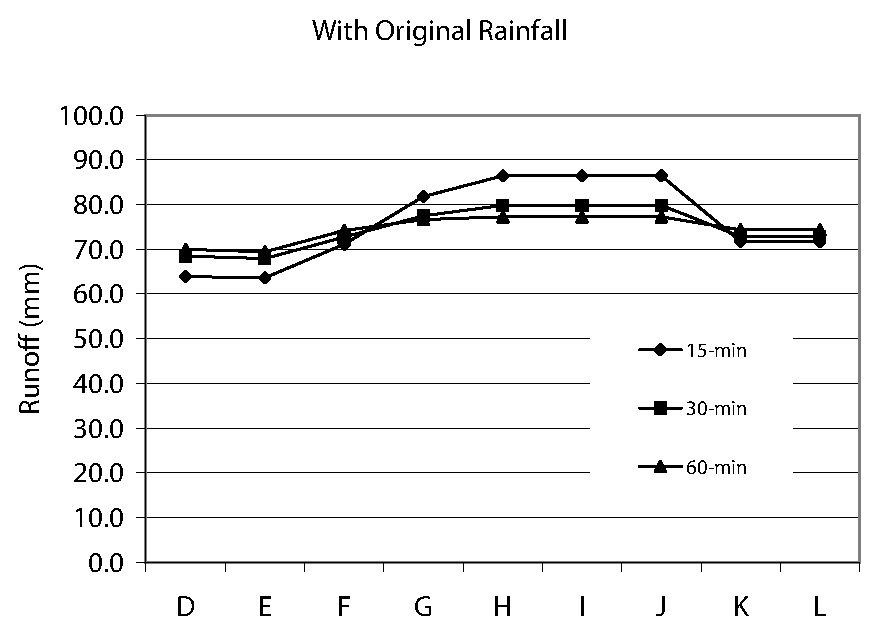
\includegraphics[width=0.49\textwidth]{./img/wepp_runoff_with_original}
    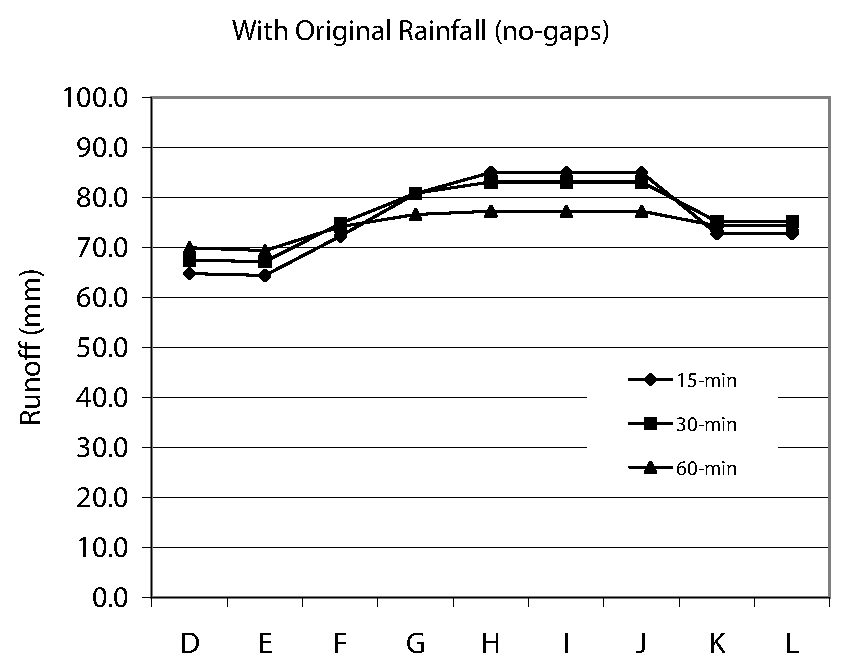
\includegraphics[width=0.49\textwidth]
{./img/wepp_runoff_with_original_nogap}\\[5mm]
    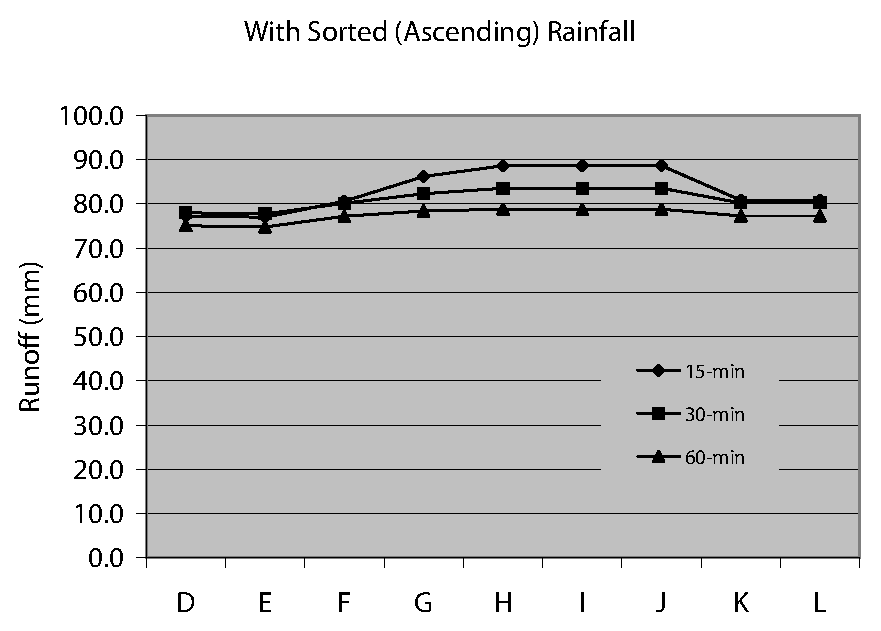
\includegraphics[width=0.49\textwidth]{./img/wepp_runoff_with_sorted_asc}
    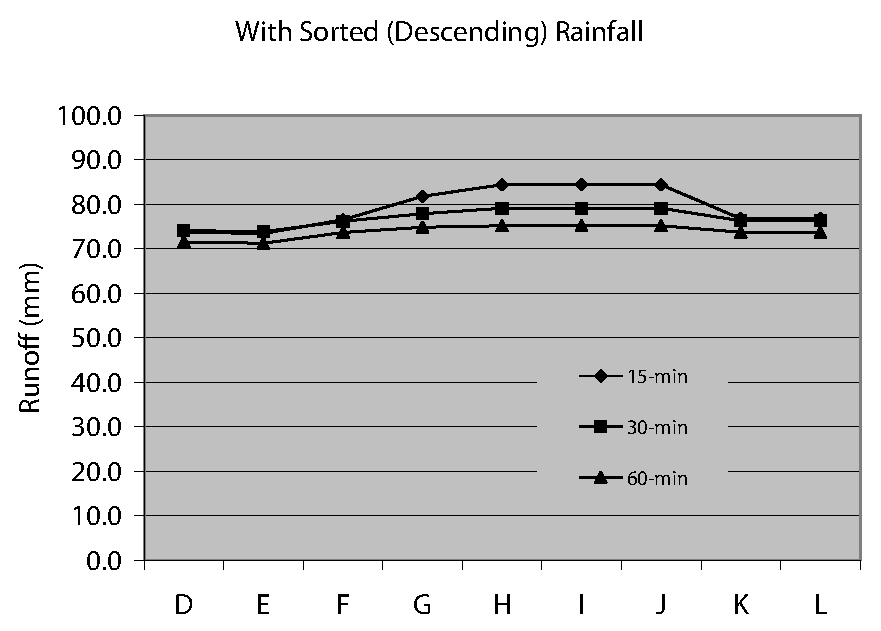
\includegraphics[width=0.49\textwidth]{./img/wepp_runoff_with_sorted_des}
  \caption{WEPP simulated runoff rates with original and sorted October rainfall
data}
  \label{fig:wepp_runoff_results}
\end{figure}

\begin{figure}[htbp]
  \centering
    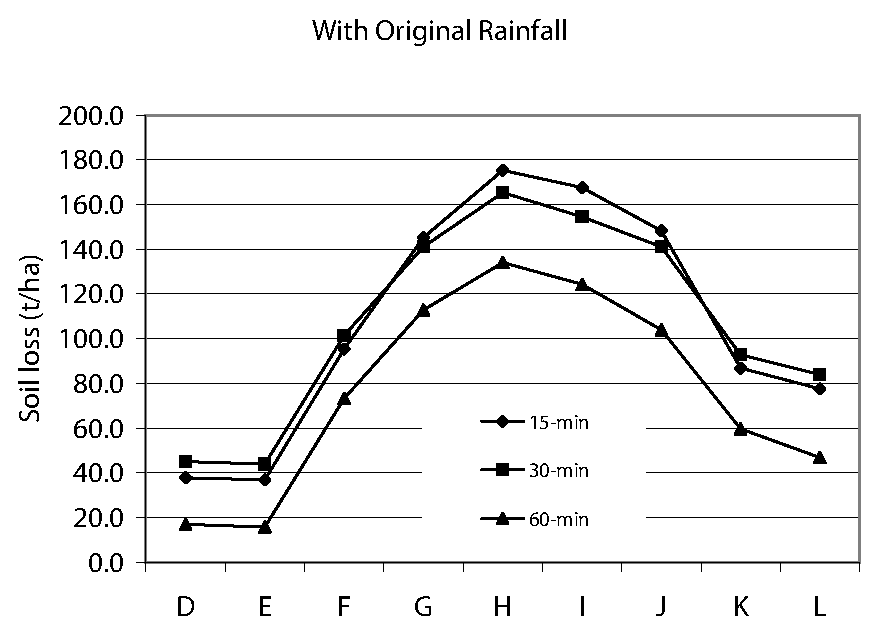
\includegraphics[width=0.49\textwidth]{./img/wepp_soilloss_with_original}
    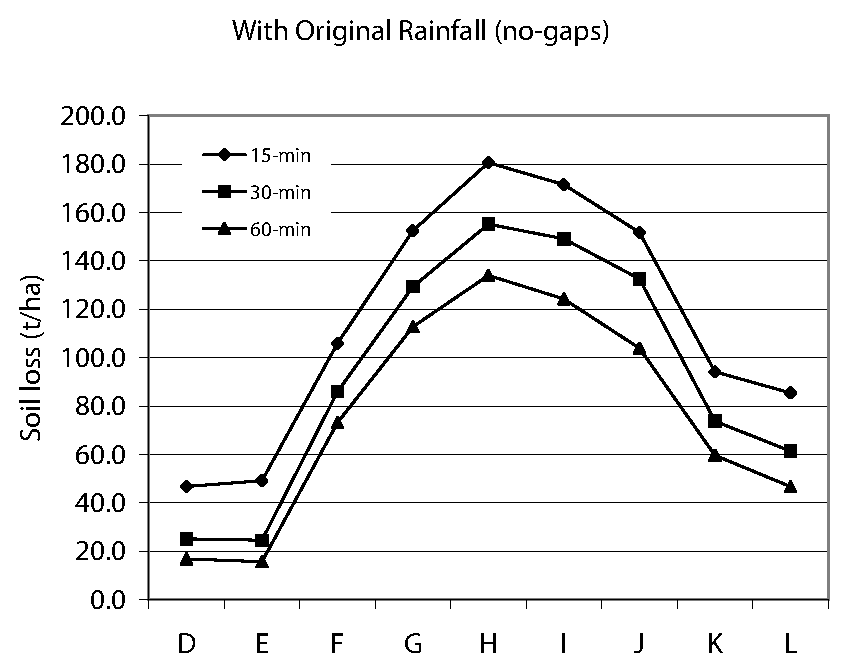
\includegraphics[width=0.49\textwidth]
{./img/wepp_soilloss_with_original_nogap}\\[5mm]
    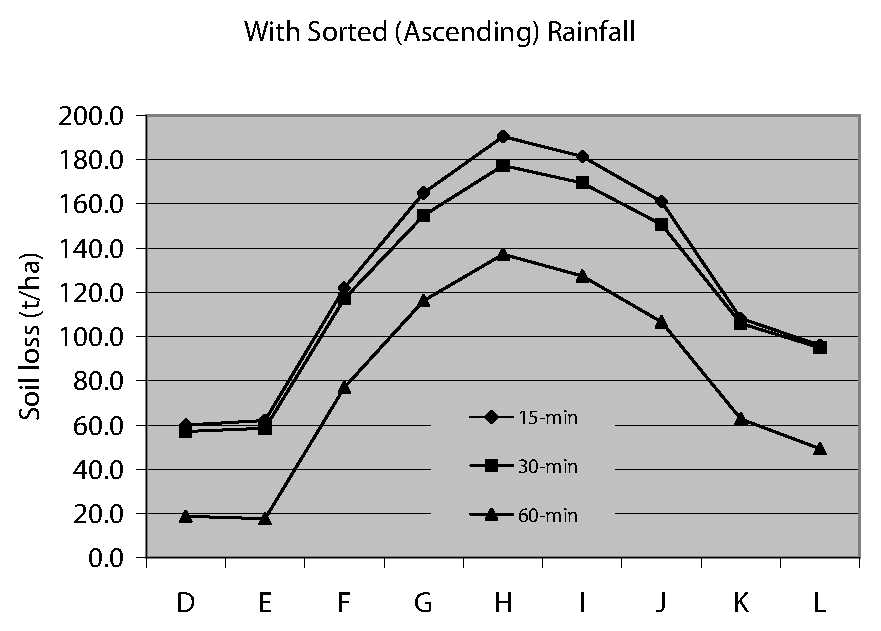
\includegraphics[width=0.49\textwidth]{./img/wepp_soilloss_with_sorted_asc}
    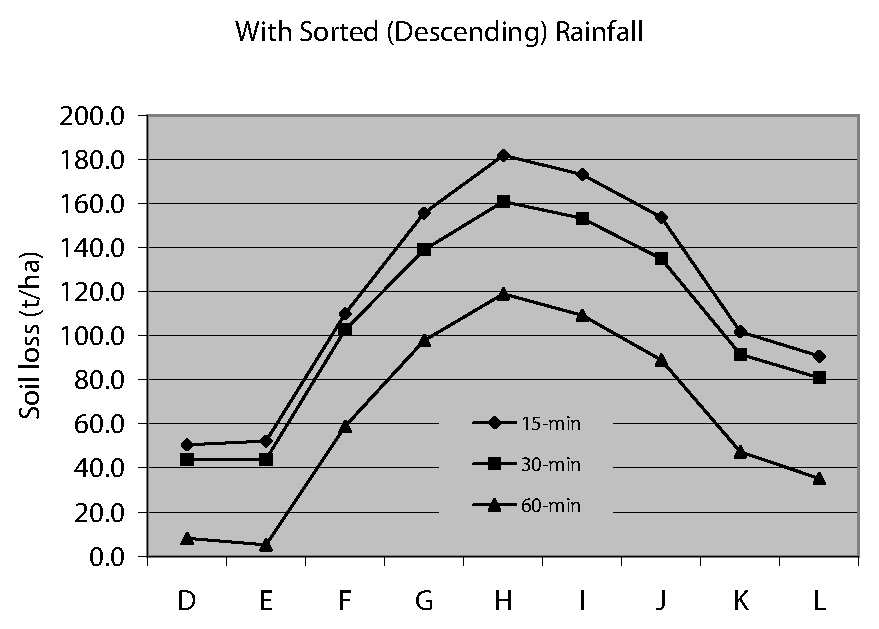
\includegraphics[width=0.49\textwidth]{./img/wepp_soilloss_with_sorted_des}
  \caption{WEPP simulated soil loss rates with original and sorted October
rainfall data}
  \label{fig:wepp_soilloss_results}
\end{figure}

\begin{figure}[htbp]
  \centering
    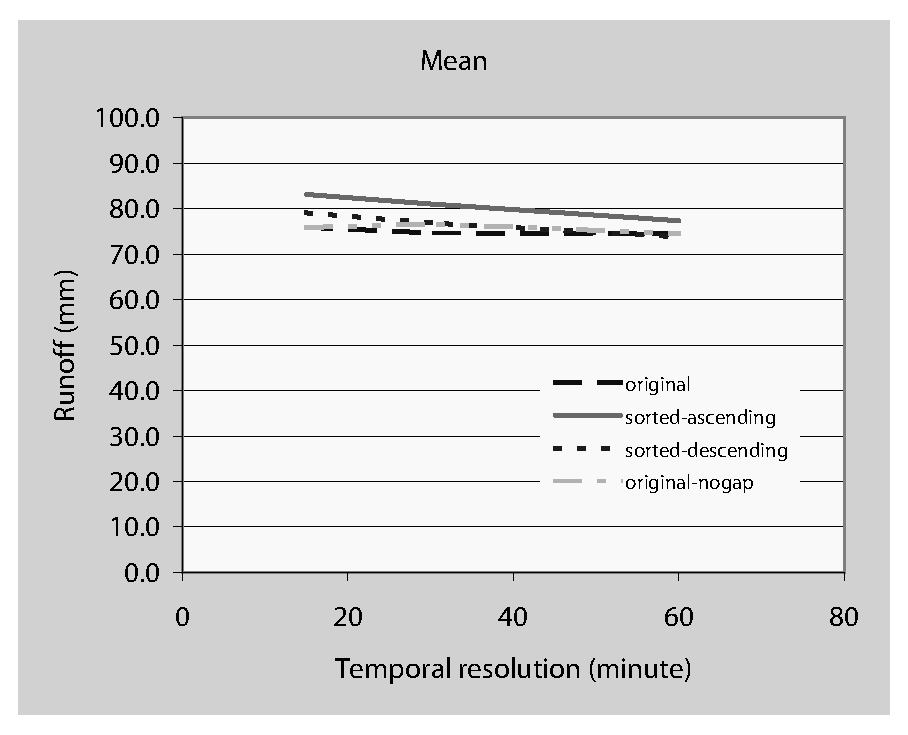
\includegraphics[width=0.49\textwidth]{./img/wepp_mean_runoff}
    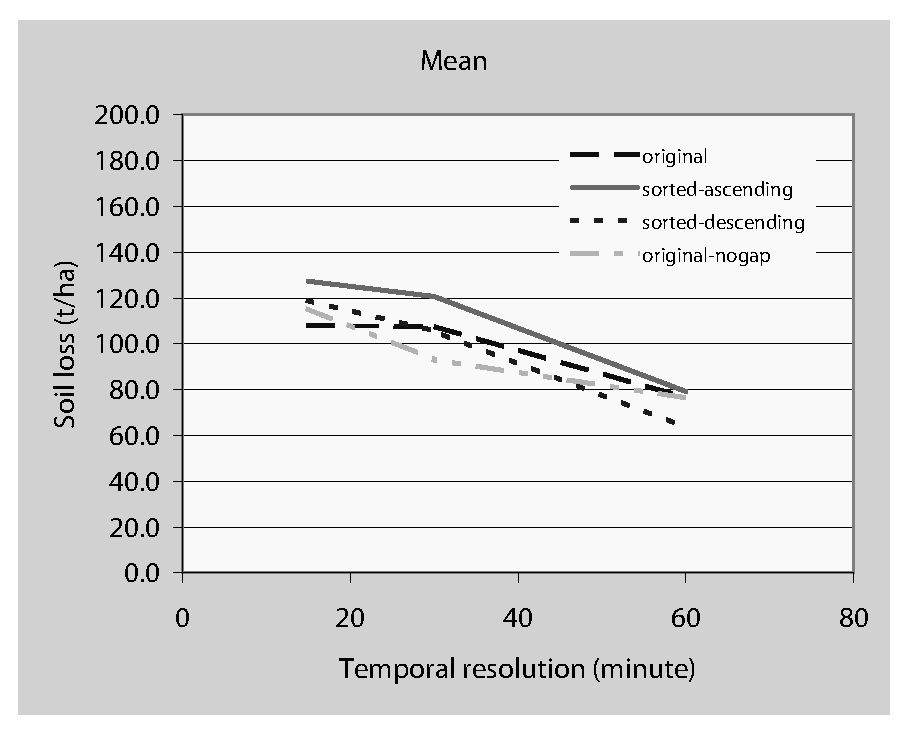
\includegraphics[width=0.49\textwidth]{./img/wepp_mean_soilloss}
  \caption{WEPP simulated mean runoff and soil loss rates with different
temporal data resolutions}
  \label{fig:wepp_mean_runoff_soilloss_diff}
\end{figure}

\begin{figure}[htbp]
  \centering
    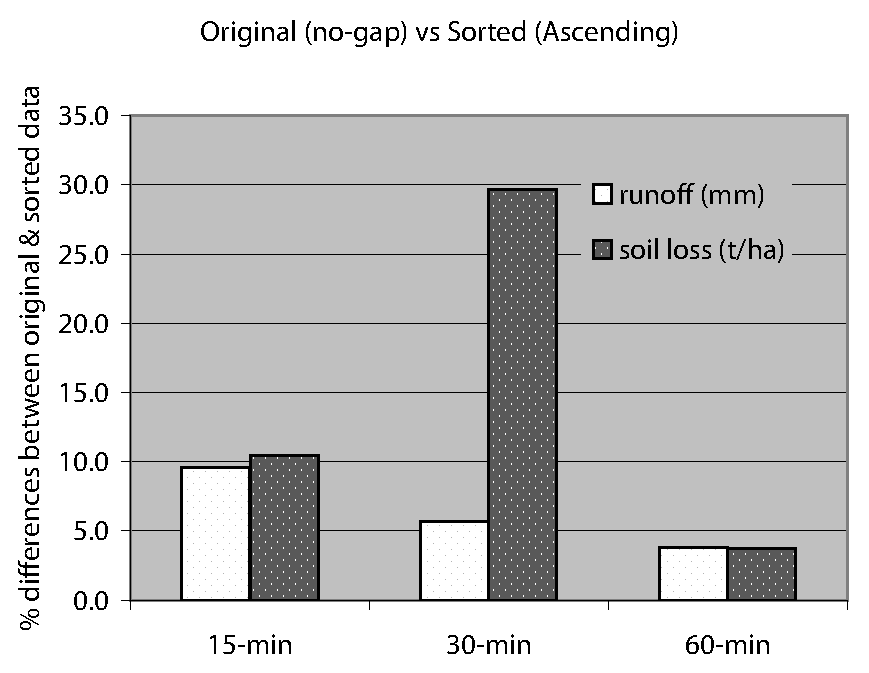
\includegraphics[width=0.49\textwidth]{./img/wepp_diff_runoff_soilloss_asc}
    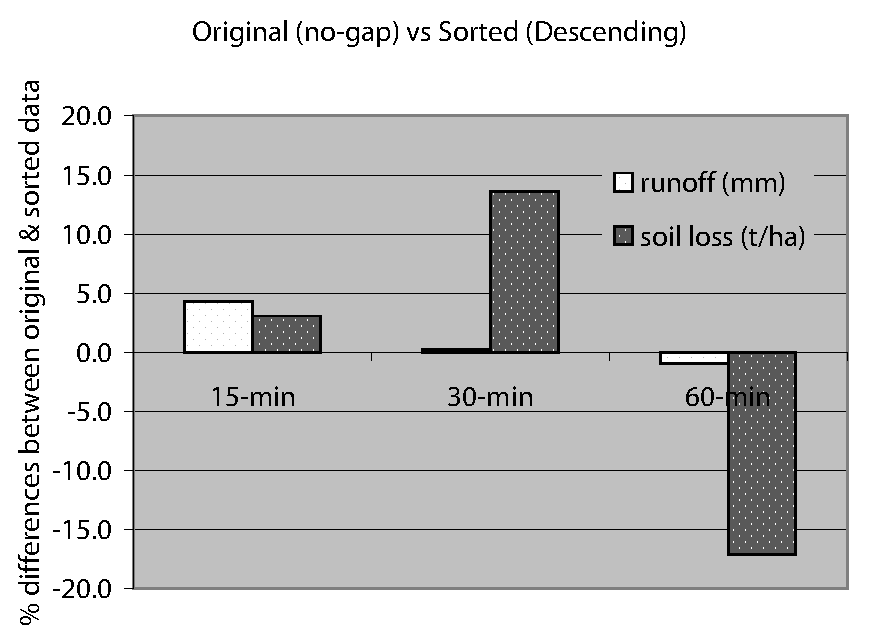
\includegraphics[width=0.49\textwidth]{./img/wepp_diff_runoff_soilloss_des}
  \caption{Changes in WEPP simulated runoff and soil loss rates using original
and sorted rainfall data for different temporal data resolution}
  \label{fig:wepp_diff_runoff_soilloss}
\end{figure}

\subsection{EUROSEM simulation}
\label{sec:EUROSEMSimulation}

\begin{sidewaystable}[htbp]
  \centering
  \small
  \caption{EUROSEM simulations with October rainfall data}
  \label{tab:EUROSEMSimulationsWithOctoberRainfallData}
    \begin{tabular}{llllllllllllll}
\toprule
\multicolumn{3}{c}{EUROSEM with October Storm} & D & E & F & G & H & I & J & K &
L & MEAN & \% $\Delta$ from original \\
\midrule
15-min & runoff & original & 62.9 & 62.9 & 63.0 & 63.2 & 63.4 & 63.3 & 63.2 &
63.0 & 63.0 & 63.1 &  \\
 & (mm) & original-nogap & 70.3 & 70.2 & 70.3 & 70.6 & 70.8 & 70.7 & 70.6 & 70.3
& 70.3 & 70.5 & \\
 &  & sorted-ascending & 82.9 & 82.7 & 83.1 & 83.2 & 83.6 & 83.4 & 83.4 & 83.2 &
83.3 & 83.2 & 31.9 \\
 &  & sorted-descending & 84.2 &  84.2 &  84.4 &  84.5 &  84.6 &  84.5 &  84.4 &
84.3 &  84.3 &  84.4 &  33.7\\
 & soil loss  & original & 19.3 & 19.3 & 26.4 & 39.1 & 59.0 & 43.9 & 36.6 & 23.3
& 22.0 & 32.1 &  \\
 & (t/ha) & original-nogap &  21.8 &  21.8 &  29.7 &  43.6 &  66.0 &  49.1 &
40.8 &  26.3 &  24.8 &  36.0 & \\
 &  & sorted-ascending & 22.5 & 22.4 & 30.7 & 46.9 & 72.5 & 53.3 & 44.3 & 27.4 &
26.0 & 38.4 & 19.8 \\
 &  & sorted-descending & 25.1 &  25.1 &  34.2 &  49.3 &  77.6 &  56.2 &  46.2 &
30.5 &  28.8 &  41.4 &  29.2\\
\midrule
30-min & runoff  & original & 69.4 & 69.3 & 69.5 & 69.6 & 69.7 & 69.6 & 69.6 &
69.5 & 69.4 & 69.5 &  \\
 & (mm) & original-nogap &  71.4 &  71.4 &  71.6 &  71.7 &  71.8 &  71.7 &  71.7
& 71.5 &  71.5 &  71.6 & \\
 &  & sorted-ascending & 80.1 & 79.9 & 80.3 & 80.4 & 80.7 & 80.6 & 80.6 & 80.4 &
80.5 & 80.4 & 15.6 \\
 &  & sorted-descending & 80.8 &  80.8 &  81.0 &  81.1 &  81.2 &  81.0 &  81.0 &
80.9 &  80.9 &  80.9 &  16.4\\
 & soil loss  & original & 21.9 & 21.8 & 29.8 & 41.5 & 64.8 & 46.5 & 38.8 & 26.5
& 25.1 & 35.2 &  \\
 & (t/ha) & original-nogap &  22.8 &  22.8 &  31.1 &  43.0 &  67.0 &  48.0 &
40.1 &  27.7 &  26.2 &  36.5 & \\
 &  & sorted-ascending & 23.7 & 23.5 & 32.1 & 44.9 & 72.5 & 51.4 & 42.2 & 28.7 &
27.2 & 38.5 & 9.4 \\
 &  & sorted-descending & 26.2 &  26.1 &  35.8 &  47.0 &  77.1 &  53.7 &  43.8 &
31.9 &  30.2 &  41.3 &  17.5\\
\midrule
60-min & runoff  & original & 74.4 & 74.4 & 74.6 & 74.6 & 74.8 & 74.7 & 74.6 &
74.5 & 74.5 & 74.6 &  \\
 & (mm) & original-nogap &  75.5 &  75.5 &  75.7 &  75.8 &  75.9 &  75.8 &  75.8
& 75.6 &  75.6 &  75.7 & \\
 &  & sorted-ascending & 78.2 & 78.1 & 78.4 & 78.5 & 78.8 & 78.7 & 78.7 & 78.5 &
78.6 & 78.5 & 5.3 \\
 &  & sorted-descending & 77.9 &  77.9 &  78.1 &  78.2 &  78.3 &  78.2 &  78.1 &
78.0 &  78.0 &  78.1 &  4.7\\
 & soil loss  & original & 23.3 & 23.2 & 31.8 & 43.5 & 69.8 & 50.2 & 40.6 & 28.3
& 26.8 & 37.5 &  \\
 & (t/ha) & original-nogap &  24.0 &  23.9 &  32.8 &  44.7 &  71.2 &  51.4 &
41.7 &  29.2 &  27.6 &  38.5 & \\
 &  & sorted-ascending & 24.2 & 24.1 & 33.0 & 44.6 & 72.3 & 51.4 & 41.8 & 29.5 &
27.9 & 38.8 & 3.4 \\
 &  & sorted-descending & 26.8 &  26.7 &  36.7 &  46.4 &  75.6 &  53.2 &  43.1 &
32.7 &  31.0 &  41.4 &  10.3\\
\bottomrule
    \end{tabular}
\end{sidewaystable}

\begin{figure}[htbp]
  \centering
    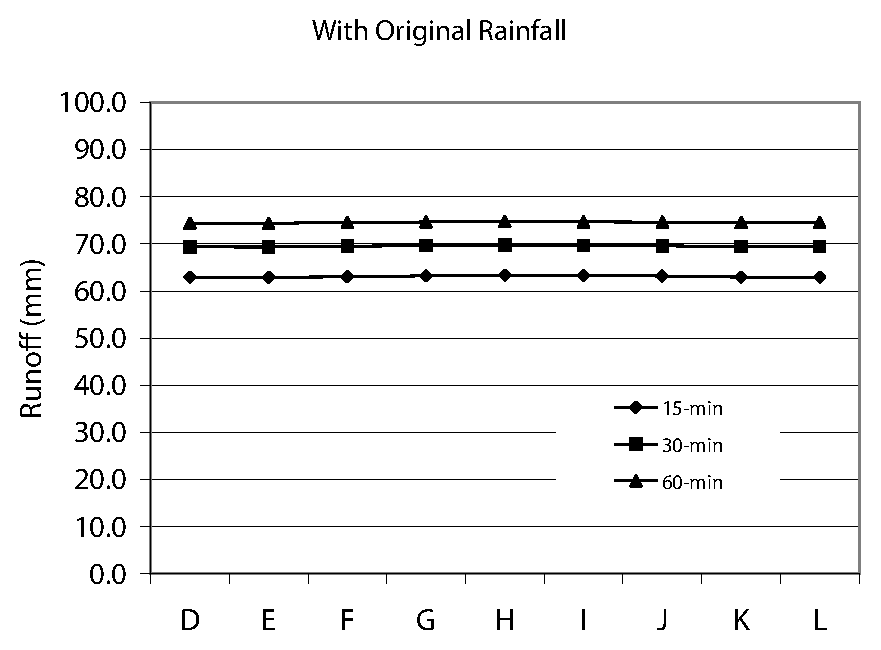
\includegraphics[width=0.49\textwidth]{./img/eurosem_runoff_with_original}
    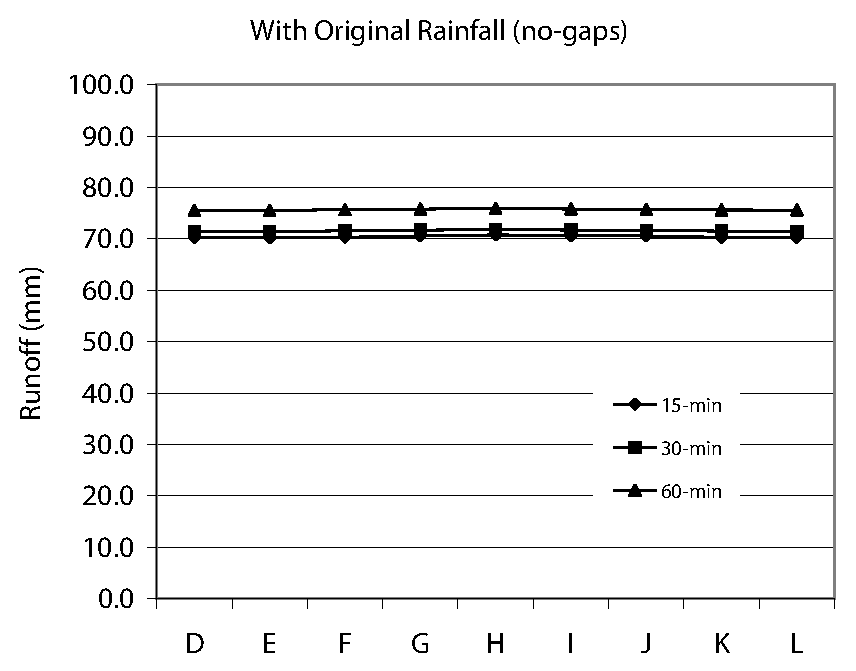
\includegraphics[width=0.49\textwidth]
{./img/eurosem_runoff_with_original_nogap}\\[5mm]
    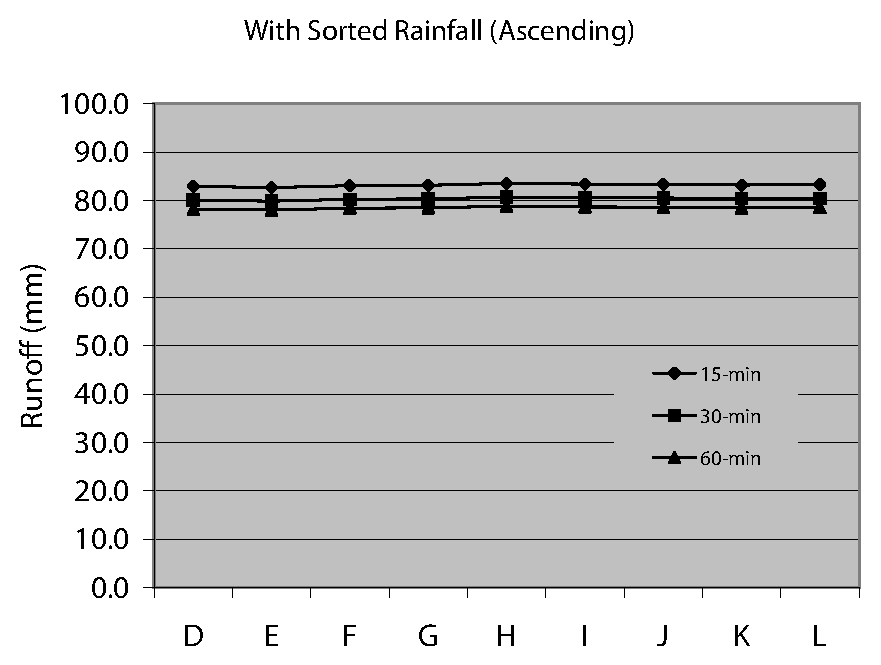
\includegraphics[width=0.49\textwidth]{./img/eurosem_runoff_with_sorted_asc}
    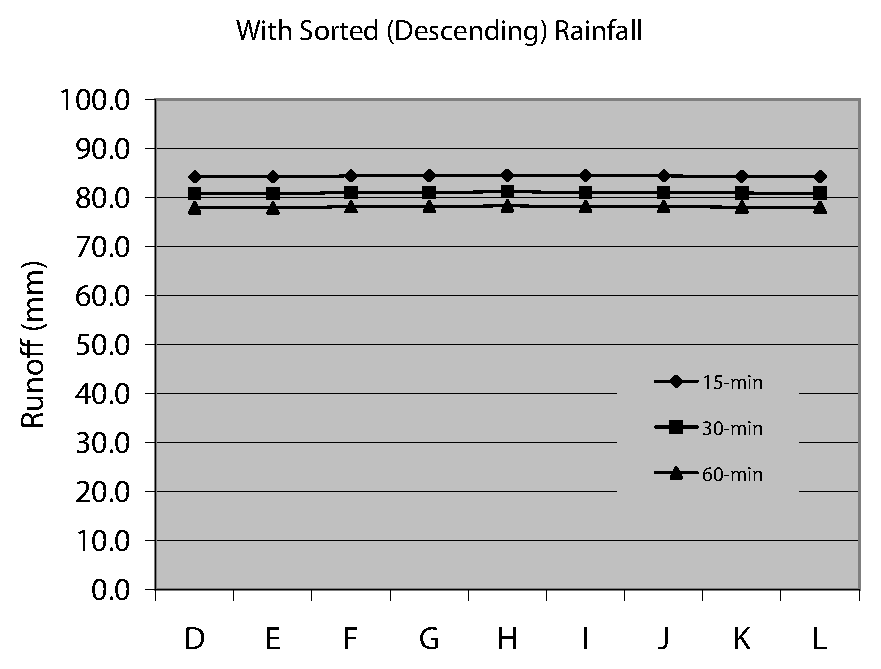
\includegraphics[width=0.49\textwidth]{./img/eurosem_runoff_with_sorted_des}
  \caption{EUROSEM simulated runoff rates with original and sorted October
rainfall data}
  \label{fig:eurosem_runoff_results}
\end{figure}

\begin{figure}[htbp]
  \centering
    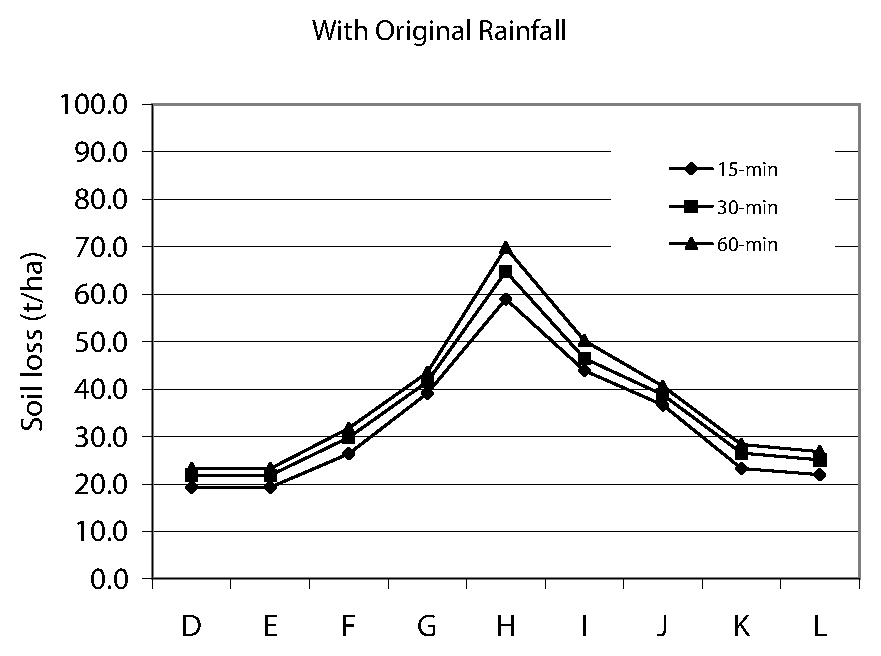
\includegraphics[width=0.49\textwidth]{./img/eurosem_soilloss_with_original}
    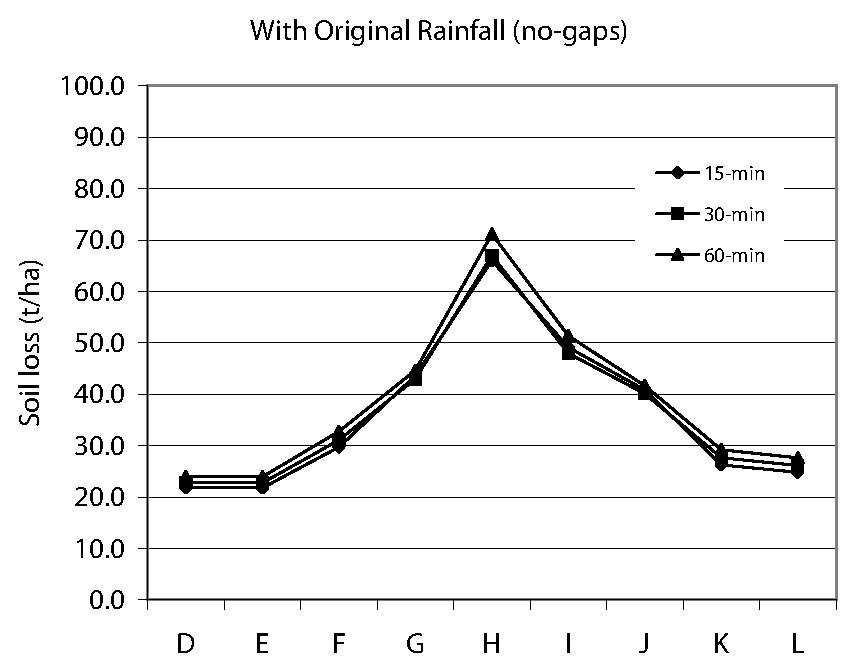
\includegraphics[width=0.49\textwidth]
{./img/eurosem_soilloss_with_original_nogap}\\[5mm]
    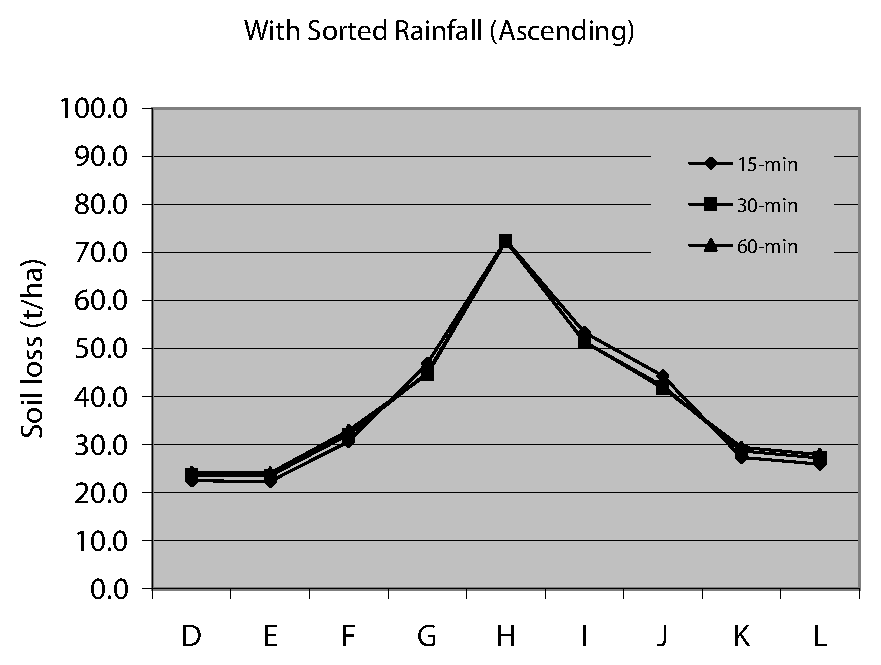
\includegraphics[width=0.49\textwidth]
{./img/eurosem_soilloss_with_sorted_asc}
    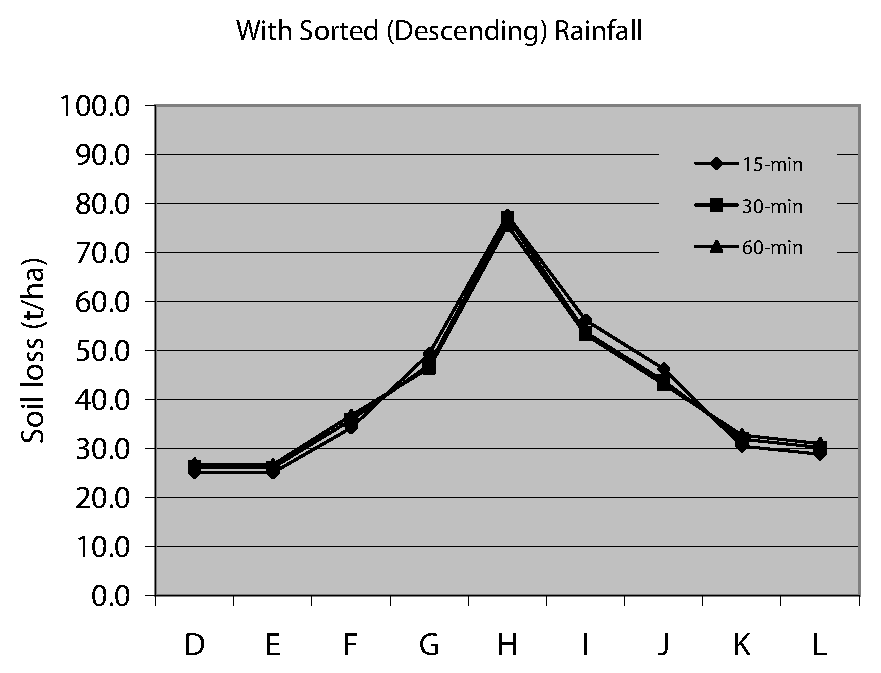
\includegraphics[width=0.49\textwidth]
{./img/eurosem_soilloss_with_sorted_des}
  \caption{EUROSEM simulated soil loss rates with original and sorted October
rainfall data}
  \label{fig:eurosem_soilloss_results}
\end{figure}

\begin{figure}[htbp]
  \centering
    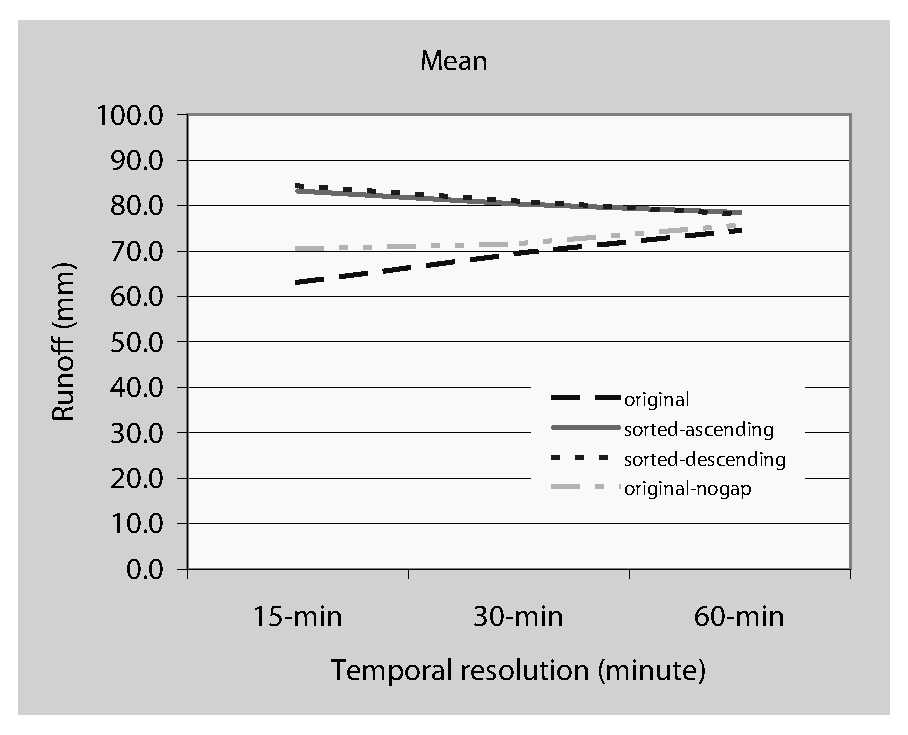
\includegraphics[width=0.49\textwidth]{./img/eurosem_mean_runoff}
    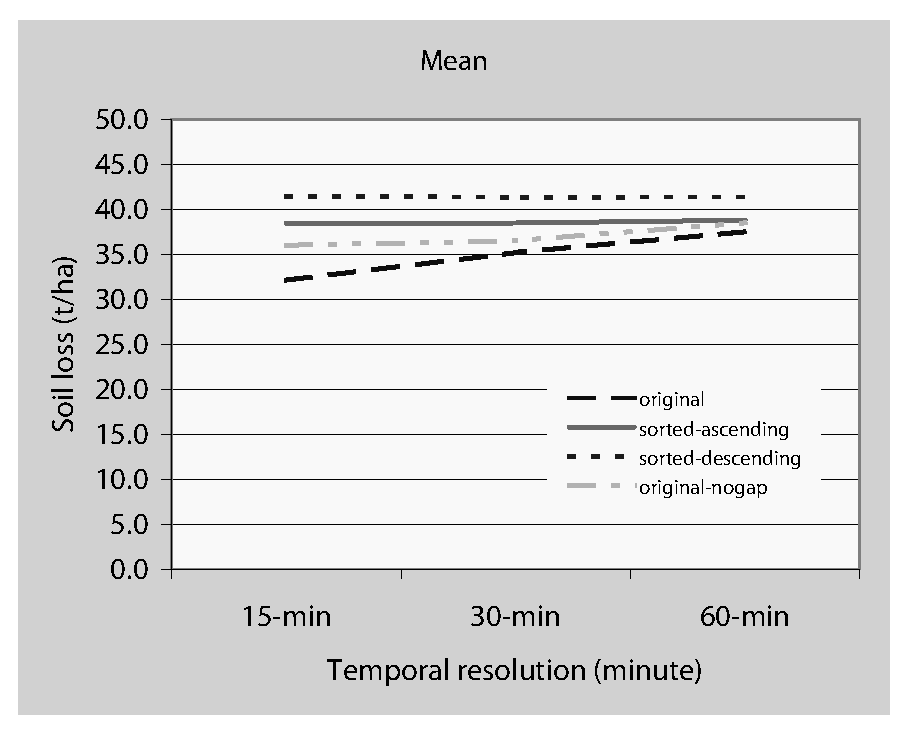
\includegraphics[width=0.49\textwidth]{./img/eurosem_mean_soilloss}
  \caption{EUROSEM simulated mean runoff and soil loss rates with different
temporal data resolutions}
  \label{fig:eurosem_mean_runoff_soilloss_diff}
\end{figure}

\begin{figure}[htbp]
  \centering
    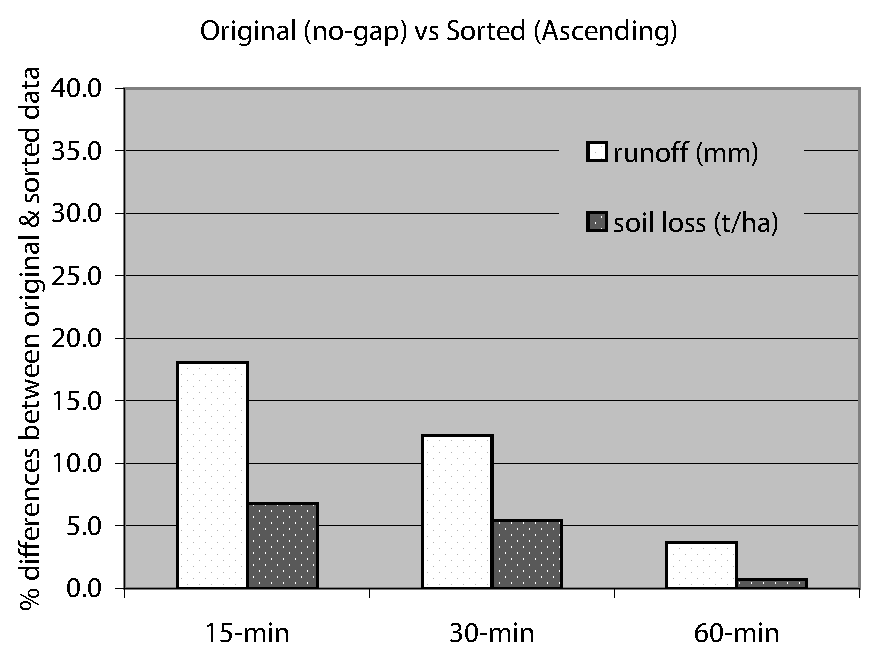
\includegraphics[width=0.49\textwidth]
{./img/eurosem_diff_runoff_soilloss_asc}
    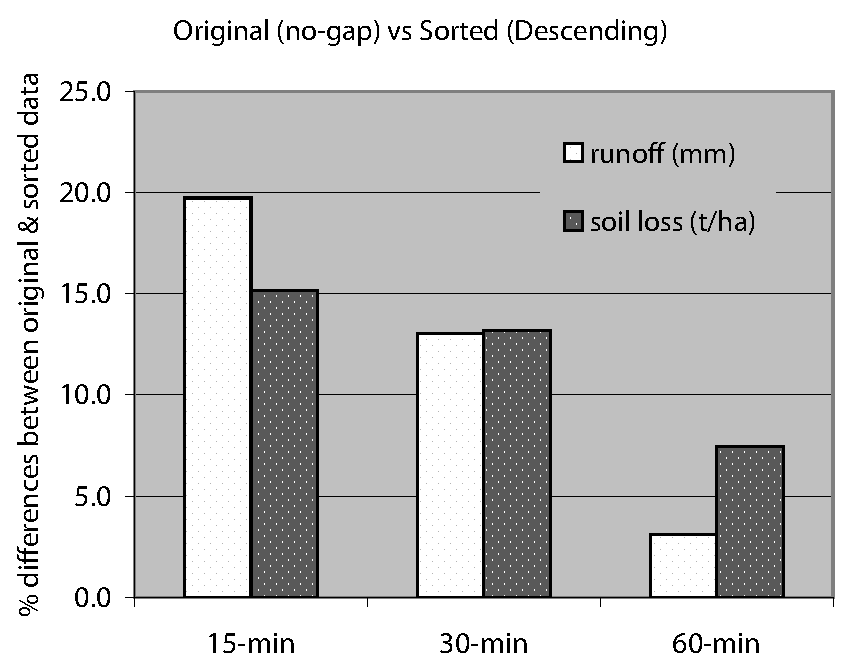
\includegraphics[width=0.49\textwidth]
{./img/eurosem_diff_runoff_soilloss_des}
  \caption{Changes in EUROSEM simulated runoff and soil loss rates using
original and sorted rainfall data for different temporal data resolution}
  \label{fig:eurosem_diff_runoff_soilloss}
\end{figure}

\section{Discussion}
\label{sec:Discussion}
Things that I need to discuss:
\begin{itemize}
  \item Only 15-, 30-, and 60-min temporal resolutions used because of the
limitation on the number of breakpoints that WEPP can take
  \item Try to minimise possible effects from other factors (gaps, rainfall
amount, duration, shape of the storm, etc.)
  \item Re-sorting the data will results in ``increasing-intensity'' storm or
``decreasing-intensity'' storm. Thus, the effects from the differences in
temporal intensity variation may be only applicable for whichever storm shape we
used, in this case ``increasing-intensity''.
  \item The differences I may see here may be the results of models' artefacts.
  \item \dots
\end{itemize}

For EUROSEM simulation, each slope has been flattened to have a uniform slope
angle.

The original rainfall data have no-rain phases which might have affected runoff
and soil loss rate simulations. This may be the case for the simulations with
sorted-descending rainfall data. From the charts (Chart1-3 in WEPP-outputs.xls),
the simulated soil loss rate with sorted-descending rainfall data show higher
soil loss rate for 15-min, similar for 30-min, and less for 60-min than the ones
with original rainfall.

Runoff and soil loss rates with sorted-ascending rainfall data and
sorted-descending rainfall data seems running parallel to each other (see
Chart1-2 in WEPP-outputs.xls).

Sorted-descending and sorted-ascending rainfall data have the same rainfall
duration as well as rainfall amount.

Thus, original without the gaps were subjected to the same simulations. The
modified original rainfall data have the same rainfall duration as sorted data.

For WEPP, rainfall data with higher bp-to-bp variability (original rainfall
data) resulted in less affected runoff and soil loss rates by temporal
resolution. -- quantify this! Runoff and soil loss rate with original rainfall
has low $\beta$ value (from $y= \beta x + \alpha$).

For EUROSEM,  rainfall data with higher bp-to-bp variability (original) showed
more affected runoff and soil loss rates by temporal resolution. -- quantify
this! Runoff and soil loss rate with original rainfall has high $\beta$ value
(from $y= \beta x + \alpha$).

Higher temporal resolution data have greater temporal variation in intensity.
These variations were reduces by ``sorting'' the same rainfall data. The data
were sorted by ascending order.

15-min resolution data showed greater differences between original \& sorted

60-min resolution data showed little differences compare to the 15-min.

Proportionally soil loss rate simulated by WEPP is affected more compared to
runoff.

+++++

15-min data generated higher runoff \& erosion rates.

Sorted data generated more runoff \& erosion.

15-min data showed greater differences between original \& sorted.

High temporal resolution resulted in greater runoff \& soil erosion rate for
both (original \& sorted).

Effects of high temporal resolution \& high temporal variation is grater for
erosion (Fig. \ref{fig:wepp_diff_runoff_soilloss}) -- are you sure? check this!

\section{Additional tests}
\label{sec:AdditionalTests}

further test with different intensity and variability

\subsection{Aims}
\label{sec:Aims}

Terms to be defined:

unsorted (original) = high (natural) breakpoint-to-breakpoint variability

sorted = low breakpoint-to-breakpoint variability

There are two way of calculating BP-to-BP Variance. One is to simply add all the
values with the +/- signs. The other is to calculate RMS (root mean square) for
the value. This will remove the orientation of the BP-to-BP variance.

I need to justify why I have used intensity (or amount) for
breakpoint-to-breakpoint variability.


\begin{table}[htbp]
  \centering
  \caption{Breakpoint-to-breakpoint variances calculated with rainfall amount
(mm)}
    \begin{tabular}{llrrr}
      \toprule
      &  & \multicolumn{1}{l}{15-min} & \multicolumn{1}{l}{30-min} &
\multicolumn{1}{l}{60-min} \\
      \midrule
      Simple Addition & Original (without no-rain phase)& -0.01 & -0.02 & -0.04
\\
      &Sorted (Ascending) & 0.1 & 0.31 & 0.92 \\
      &Sorted (Descending) & -0.1 & -0.31 & -0.92 \\
      \midrule
      Root Mean Square &Original (without no-rain phase)& 2 & 3.56 & 5.44 \\
      &Sorted (Ascending) & 0.2 & 0.45 & 1.16 \\
      &Sorted (Descending) & 0.2 & 0.45 & 1.16 \\
      \bottomrule
    \end{tabular}
  \label{b2b_amount}
\end{table}

It is more appropriate to use intensity in calculating Breakpoint-to-breakpoint
variance. When amount is used, for example 15-min data, breakpoint-to-breakpoint
variance will be smaller than 60-min data because 15-min data has generally
smaller rainfall amount for a Breakpoint-to-breakpoint time period in comparison
to 60-min. Thus, direct comparison does not give valid comparison. However, when
intensity is used, temporal resolution for each amount is considered so that
breakpoint-to-breakpoint variance can be compared. Therefore, rainfall intensity
is used for calculating breakpoint-to-breakpoint variances for each temporal
resolution.

\begin{table}[htbp]
  \centering
  \caption{Breakpoint-to-breakpoint variances calculated with rainfall intensity
(mm/hr)}
  \label{b2b_intensity}
    \begin{tabular}{llrrr}
      \toprule
       &  & \multicolumn{1}{l}{15-min} & \multicolumn{1}{l}{30-min} &
\multicolumn{1}{l}{60-min} \\
      \midrule
      Simple Addition & Original (without no-rain phase)& -0.05 & -0.05 & -0.04
\\
       & Sorted (Ascending) & 0.39 & 0.62 & 0.92 \\
       & Sorted (Descending) & -0.39 & -0.62 & -0.92 \\
      \midrule
      Root Mean Square & Original (without no-rain phase)& 8.22 & 7.13 & 5.45 \\
       & Sorted (Ascending) & 0.81 & 0.89 & 1.16 \\
       & Sorted (Descending) & 0.81 & 0.89 & 1.16 \\
      \midrule
      Mean of Sum of & Original (without no-rain phase) & 6.19 & 5.67 & 4.47 \\
      Absolute Values & Sorted (Ascending)& 0.39 & 0.62 & 0.92 \\
       & Sorted (Descending)& 0.39 & 0.62 & 0.92 \\
      \bottomrule
    \end{tabular}
\end{table}

Original -- RMS\\
This result is something that I have expected to see. Shorter the temporal
resolution of data,  greater the BP-to-BP variances.

Asc. \& Des -- RMS\\
These are somewhat interesting. There must be reasons to explain this. Why
greater BP-to-BP variance for the longer temporal resolution data?

The total value of the variance for the 15-min data is greater than 60-min data.
However, mean becomes smaller for the 15-min data than 60-min data because of
the total number of data points for 15-min data.

Maximum breakpoint-to-breakpoint variability can be obtained by sorting the
storm data (to ascending and descending either way) and calculating
breakpoint-to-breakpoint variability. Because the breakpoint comes in next will
have the smallest possible breakpoint-to-breakpoint variability and so on.

In contrast, maximum breakpoint-to-breakpoint variability can be achieved by
taking one breakpoint data from the either end of the sorted data, and stack
them in alternating manner.% For example, if we have rainfall data consists of 6
%breakpoints as below:
%
% Original breakpoint data (mm/min): 1 2 3 9 4 5
%
% Sorted minimum variability can be obtained by sorting the data to: 1 2 3 4 5
%9.
%
% Maximum breakpoint-to-breakpoint can be obtained when the data has alternating
%order: 1 9 2 5 3 4.
%
%
%
% 1. Methods
%
%   +/- 10 or less mm for each breakpoint
%   Changes amounts
%   But the variability will be the same (check!)
%
%   +/- 10 or less \% for each breakpoint
%   Changes amounts
%   Also changes variability? (check!)
%
% Original MSA(Mean of Sum of Absolute) -- for Tony's question
%
% Sorted 15-60 may or may not important. They may have opposite pattern, but it
%is important to compare to ascending vs. descending -- effects of shape g the
%storm.

%\nolinenumbers
